%%---------------------------------------------------------------------------%%
%% draco-release.tex
%% Thomas M. Evans
%% $Id$
%%---------------------------------------------------------------------------%%
\documentclass[11pt]{nmemo}
\usepackage[centertags]{amsmath}
\usepackage{amssymb,amsthm,graphicx}
\usepackage[mathcal]{euscript}
\usepackage{tmadd,tmath}
\usepackage{cite}

%%---------------------------------------------------------------------------%%
%% DEFINE SPECIFIC ENVIRONMENTS HERE
%%---------------------------------------------------------------------------%%
%\newcommand{\elfit}{\ensuremath{\operatorname{Im}(-1/\epsilon(\vq,\omega)}}
%\msection{}-->section commands
%\tradem{}  -->add TM subscript to entry
%\ucatm{}   -->add trademark footnote about entry

\newcommand{\draco}{{\normalfont\normalsize\sffamily Draco}}
\newcommand{\milagro}{{\normalfont\normalsize\sffamily Milagro}}
\newcommand{\solon}{{\normalfont\normalsize\sffamily Solon}}
\newcommand{\capsaicin}{{\normalfont\normalsize\sffamily Capsaicin}}

\newcommand{\cfour}{{\normalfont\normalsize\sffamily c\footnotesize 4}}
\newcommand{\dsxx}{{\normalfont\normalsize\sffamily ds\raisebox{.2ex}
  {\scriptsize ++}}}

\newcommand{\stable}{{\normalfont\normalsize\ttfamily last\_stable}}

%%---------------------------------------------------------------------------%%
%% BEGIN DOCUMENT
%%---------------------------------------------------------------------------%%
\begin{document}

%%---------------------------------------------------------------------------%%
%% OPTIONS FOR NOTE
%%---------------------------------------------------------------------------%%

\toms{Distribution}
%\toms{Joe Sixpak/XTM, MS B226}
\refno{XTM:99--36 (U) Rev. 2}
\subject{Draco Release Policy and Procedures}

%-------NO CHANGES
\divisionname{Applied Theoretical \& Computational Physics Div.}
\groupname{X-TM:Transport Methods Group}
\fromms{Thomas M. Evans/XTM D409}
\phone{(505)665--3677}
\originator{tme}
\typist{tme}
\date{May 26, 1999}
%-------NO CHANGES

%-------OPTIONS
%\reference{NPB Star Reimbursable Project}
%\thru{P. D. Soran, XTM, MS B226}
%\enc{list}      
%\attachments{list}
%\cy{list}
%\encas
%\attachmentas
%\attachmentsas 
%-------OPTIONS

%%---------------------------------------------------------------------------%%
%% DISTRIBUTION LIST
%%---------------------------------------------------------------------------%%

\distribution {
  XTM MS D409:\\ 
  J.E. Morel, XTM MS D409\\ 
  G.L. Olson, XTM MS D409\\ 
  J.M. McGhee, XTM MS D409\\ 
  H.G. Hughes, XTM MS D409\\ 
  B.T. Adams, XTM MS D409\\
  T.M. Evans, XTM MS D409\\ 
  M.G. Gray, XTM MS D409\\ 
  M.L. Hall, XTM MS D409\\ 
  S.D. Pautz, XTM MS D409\\ 
  R.M. Roberts, XTM MS D409\\ 
  S.A. Turner, XTM MS D409\\ 
  T.J. Urbatsch, XTM MS D409\\
  T.A. Wareing, XTM MS D409\\
  J.S. Warsa, XTM MS D409\\
}

%%---------------------------------------------------------------------------%%
%% BEGIN NOTE
%%---------------------------------------------------------------------------%%

\opening

\section{Revision History}

\subsection*{Rev. 2 - Nov. 4, 2010}
\begin{itemize}
\item Remove discussion of the \stable\ tag as this is not longer part
  of our normal practice.
\item Add requirement for 80\% code coverage by unit tests.
\end{itemize}

\section{Introduction}

The purpose of this memo is to outline the release policy and
procedures for \draco\ and \draco\ packages.  These procedures should
also apply to \draco-clients such as \capsaicin, \solon\ and \milagro.
We require release numbers in order to maintain quality control, code
reference, and project planning sanity in CCS--2 code projects.
\draco\ products are version-controlled by {\bf cvs} tags.  Thus,
releases of a particular code are shipped using an appropriate
\texttt{cvs export} command.

This memo contains two primary sections. \S~\ref{sec:policy} covers
release policy and \S~\ref{sec:procedures} reviews the mechanics used
to produce a release.  An Overview (\S~\ref{sec:overview}) and Summary
(\S~\ref{sec:summary}) are also provided.  Section~\ref{sec:policy} on
release policies contains information on the following topics:
\begin{enumerate}
\item the release policy for \draco-components;
\item the release policy for \draco.
\end{enumerate}
Section~\ref{sec:procedures} outlines the procedures for releasing
\draco\ and \draco-components.  In this section we will:
\begin{enumerate}
\item explain a general numbering scheme for \draco\ project releases;
\item show how to tag \draco\ package releases;
\item show how to tag \draco;
\item explain how to handle bugs in a particular \draco\ release.
\end{enumerate}
Adherence to these policies will expedite code reviews in the \draco\ 
project and will present a clean interface to outside users.
Deviations from policies described herein are allowed under special
circumstances as judged by the \draco\ project team.  The \draco\ 
release procedure heavily utilizes the {\bf cvs} version control
system.  Thus, \draco\ developers should peruse the {\bf cvs}
manual~\cite{cvs} to become intimate with its controls and use.

%%---------------------------------------------------------------------------%%

\section{Overview}
\label{sec:overview}

Historically, \draco\ evolved as a loose collection of individual
packages bound by a common build-system.  While \draco\ is more
tightly integrated in its present incarnation, \draco\ development
still concentrates on individual packages.  At this point, we will
illuminate some terminology that will be used throughout this
memorandum.  Essentially, \draco\ is a directory tree; thus, any
grouping of files that shares a common purpose is a \draco\ 
\latin{component}.  Examples of \draco\ components are
\texttt{draco/src/c4/} and \texttt{draco/config/}.  A \draco\ 
component that lives under \texttt{draco/src/} is a \draco\ 
\latin{package}.  Examples of \draco\ packages are \dsxx\ and \cfour.
Hence, packages are also \draco\ components.

\draco-clients are code systems that use \draco\ components.
\capsaicin, \solon\ and \milagro\ are \draco-clients.
\draco\ products refer to anything produced from the
\draco\ source-code tree.  On a final note, packages are often used in
a supra-\draco\ sense.  Often \milagro\ and \solon\ are referred to as
packages.  These are fundamentally different than \draco\ packages.
While we try to keep these distinctions firmly in place, one must
often derive the meaning of package from context.

Historically, the general release policy in \draco\ is to separate the
package release number from the \draco\ release number.  This approach
allowed \draco\ to have regular releases without waiting for
individual packages to get to the next release point.  For example, if
the \dsxx\ package is migrating from \texttt{ds++-1\_5\_0} to
\texttt{ds++-1\_6\_0} when \draco\ is ready for release, the
\draco\ team can release a version of \draco\ that includes
\texttt{ds++-1\_5\_0}.  If \draco\ releases are required to wait for
all packages to move forward to the next release point then the
release of \draco\ might be unnecessarily delayed.  Separating the
\draco\ and \draco\ package release numbers eased the pressure on
\draco\ package developers who might otherwise delay \draco\ releases.
More recently, \draco\ package numbers are fully synchronized with the
\draco\ release number.  This change was made because \draco\ is
relatively small and the flexibility described above wasn't usually
necessary.

A typical release of \draco\ is illustrated in
Fig.~\ref{fig:drelease}.  Each package in \draco\ is at a closure
point that is indicated by a release tag. At the time of the
\draco\ release, the package numbered release tag is concurrent with a
tag.  The tag indicates that the package is in a stable, robust
condition.  This provides a simple model for bug fixes and forward
development.  Release dates for \draco\ and \draco\ packages are
decided by \draco\ project developers as explained in
\S~\ref{sec:policy}.
\begin{figure}[ht!]
  \centerline{\includegraphics{drelease.eps}}
  \caption{Schematic figure of a sample \draco\ release.  Release
    number formats are explained in \S~\ref{sec:rel_num}.}
  \label{fig:drelease}
\end{figure}

%%---------------------------------------------------------------------------%%
 
\section{Draco Release Policies}
\label{sec:policy}

The \draco\ release policy is a set of general requirements that
controls the process of software release in the \draco\ code system.
To start, we will write down the software release policies for \draco.
Afterwards, we describe these policies in more detail.  The policies
dictating the \draco\ release process are purposely sparse.  Because
the \draco\ development team is small, only a small set of general
policies are required.  Additionally, these policies may be waived in
special circumstances by the \draco\ development team.

The \draco\ release policies are:
\begin{enumerate}
\item Each file in \draco\ will have at least a \draco-level tag.  The
  \draco\ tag is a numbered release tag that refers to a fully-stable,
  released version of \draco.
%% \item Package files in \texttt{draco/src/} will have numbered release
%%   tags in addition to the common tags.
%% \item \draco\ build-system components (\texttt{config/},
%%   \texttt{tools/}, and \texttt{templates/}) will have numbered release
%%   tags in addition to the common tags.
\item Additional \draco\ components such as \texttt{doc/} and
  \texttt{draco\_www} may or may not have tags in addition to the
  common tags.  This is a discretionary policy of the \draco\ team and 
  principal developers of the component.
\item \draco\ release dates are determined by the \draco\ development
  team.  To qualify for numbered release the following conditions must 
  be satisfied:
  \begin{itemize}
  %% \item All components in \draco\ must be in a tagged \stable\
  %%   condition.
  \item All components that maintain individual numbered release tags
    should be at a numbered release.
  \item All components must pass their respective suite of
    regression tests.
  \item Each component must have its own unit tests that cover 70\% of
    the component code base.
  \item Each component must compile without error or warning using the
    build system standard compile flags.  It is recommended that code
    be configured with \texttt{--enable-all-warnings
      --enable-glibcxx-debug} and all warnings be eliminated before
    the release.
  \item \draco\ must pass a code review that validates the release.
    The review team will include, at a minimum, all \draco\ developers
    that have contributed to any components since the last \draco\ 
    release.
  \end{itemize}
%% \item For a component to be placed in a \stable\ state the
%%   following conditions must be satisfied:
%%   \begin{itemize}
%%   \item The component must pass its regression tests.
%%   \item If the component is subject to numbered release tags, it
%%     should receive a new numbered tag concurrent with its \stable\ 
%%     tag. 
%%   \item All other \stable\ \draco\ components that depend upon this
%%     component must pass their regression tests.
%%   \end{itemize}
\item The major numbers on \draco\ numbered release tags should
  correspond to the {\bf cvs} revision numbers.  This only applies to
  \draco\ components that have numbered release tags.
\item \draco\ code packages should have a \texttt{release()} function
  that can be called from the package library.  This function returns
  a \texttt{std::string} of the numbered release tag.
\item No non-\draco\ tags should exist in \draco\ components that sit
  under the \texttt{draco/} directory in \texttt{\$CVSROOT}.
\end{enumerate}
We will now explain these policies in more detail.

%% \subsection{Draco Tagging Strategy}
%% \label{sec:stable-tag}

%% To implement the policies laid out above, we have developed the
%% concept of a \stable\ tag.  Consider a fictional representation of
%% \draco\ as illustrated in Fig.~\ref{fig:tag-strategy}.  The \stable\ 
%% tag is used
%% \begin{figure}[ht!]
%%   \centerline{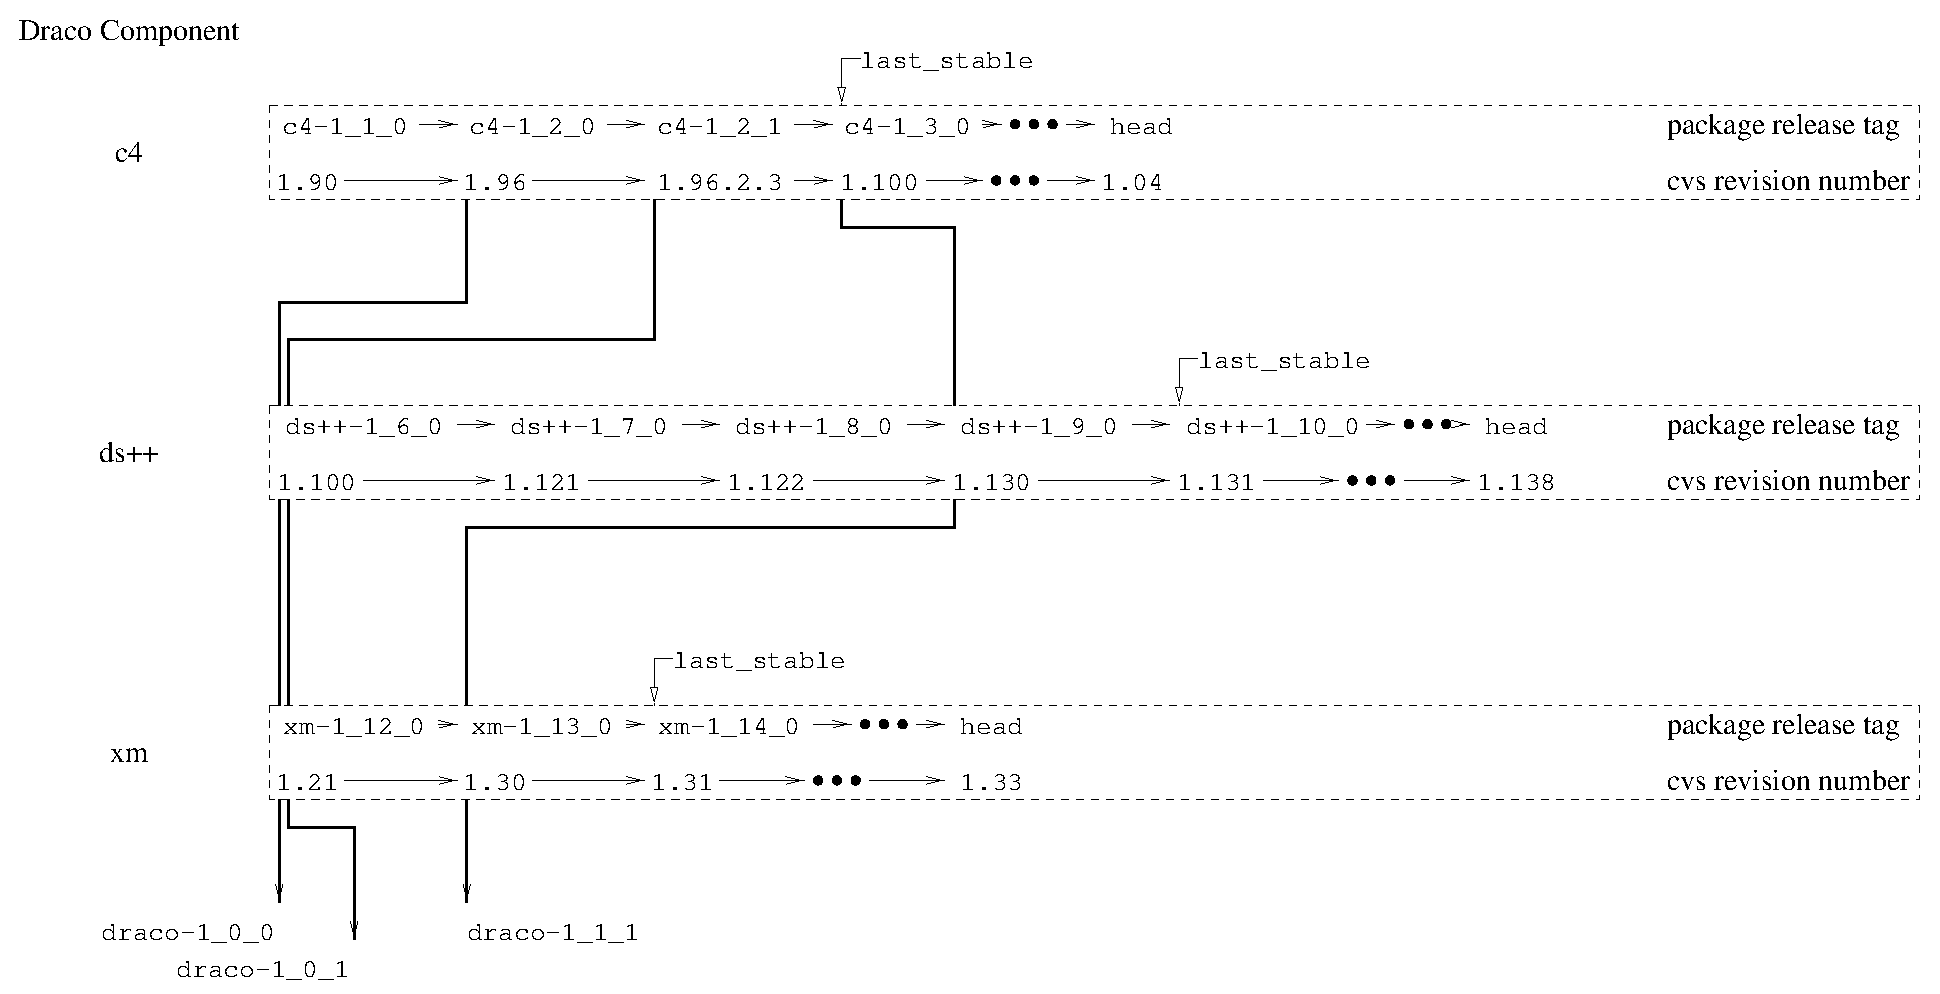
\includegraphics[width=6.5in]{tag-strategy.eps}}
%%   \caption{{\bf cvs} tagging history for a fictional representation of 
%%     \draco.  The \stable\ tag always points to the last stable release 
%%     of a particular package.}
%%   \label{fig:tag-strategy}
%% \end{figure}
%% to point to the last viable version of each package.  By viable, we
%% mean that when the \stable\ tag was assigned the package
%% \begin{enumerate}
%% \item passed its regression tests, and
%% \item all packages that depend on it have passed their regression
%%   tests.
%% \end{enumerate}
%% Thus, by checking out a \stable\ tagged version of code, one is
%% nearly guaranteed that the package works the way that the code
%% developers designed it.

%% There are some subtleties involved with the \stable\ tag that should
%% be explained.  First, the \stable\ tag is intended for the timely
%% resolution of code conflicts.  Assume that developer D is working on
%% \dsxx\ and developer C is working on \cfour\ as illustrated in
%% Fig.~\ref{fig:ab}.  C checks out the \stable\ version of \dsxx\ and
%% \begin{figure}
%%   \centerline{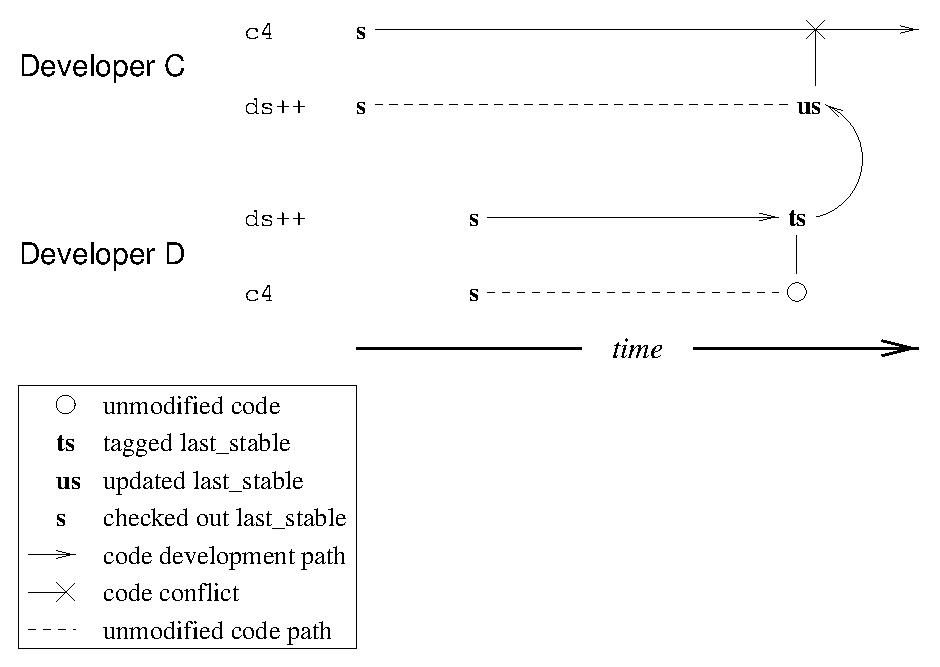
\includegraphics[width=5in]{AB.eps}}
%%   \caption{Illustration of \stable\ conflicts between packages.}
%%   \label{fig:ab}
%% \end{figure}
%% begins to modify \cfour.  In the meantime D checks out, modifies,
%% tests, and updates \dsxx\ to a new \stable\ version.  Furthermore, D
%% has properly followed \draco\ policy by testing the \stable\ version
%% of \cfour\ with his/her new head revision of \dsxx.  What can happen
%% in this instance is that the new \stable\ \dsxx\ can break C's head
%% revision of \cfour.  However, this is exactly the point of using
%% \stable\ tags during development.  In the process of bringing
%% respective versions of packages to a \stable, releasable state,
%% developers working on complementary packages are forced to communicate
%% with each other to resolve code conflicts.  The nefarious condition of
%% resolving multiple conflicts between many packages before a release,
%% which results when many developers work independently, is avoided.
%% This policy should drastically improve the stability and efficiency of
%% the \draco\ development cycle.

%% As a follow-up to the above example, we note that the development
%% system in \draco\ has several indicators for spotting possible
%% conflicts.  The first is {\bf cvs}.  Both C and D should know from
%% commit logs that \dsxx\ and \cfour\ are in a development stage.
%% Additionally, personal communication within the group should let all
%% developers know who is working on what.  Thus, the \stable\ tagging
%% policy is simply one of a number of redundant checks that ensures
%% quality and stability in \draco.

%% The \stable\ tag also significantly reduces the complexity of releasing
%% \draco.  As explained in \S~\ref{sec:procedures}, a \draco\ release is 
%% performed by checking out all of the \stable\ components of \draco.  A 
%% final test needs to be run to ensure that all the regression tests
%% pass.  \draco\ can then be given a new release tag.

%% Finally, we reemphasize that the \stable\ tag should be concurrent
%% with a numbered release for \draco\ components that have their own
%% numbered release tags.  For example, \draco\ packages have their own
%% numbered release tags, and the \stable\ tag will always point to the
%% last numbered release of a particular package.  \draco\ components
%% that do not have separate numbered release tags have no requirements
%% on \stable\ tags with the following exception.  At \draco\ release
%% points, \stable\ tags must be concurrent with the \draco\ tag.
%% Components that do not have numbered release tags separate from the
%% main \draco\ tag are not meant to change much from one \draco\ release
%% to the next.  Components in this category include files under the main
%% \draco\ directory such as \texttt{configure.in},
%% \texttt{README.draco}, and so forth.

\subsection{Draco Components}

\draco\ components include both files contained in a subdirectory and
free files.  Free files include the build-system infrastructure files
under \texttt{draco/}, \texttt{draco/src/},
\texttt{draco/environment/} and \texttt{draco/doc/}.  Packages under
the \texttt{draco/src/} directory are components.  The
\texttt{draco/config/} directory is a component.  All
\draco\ components have at least a \draco-level tag.  Certain
components, including packages and build-system components such as
\texttt{draco/config/}, have their own numbered tags in addition to
the two aforementioned tags.  Additional components may or may not
have numbered release tags depending upon their purpose.  The decision
about whether to provide a numbered tag for these additional
\draco\ components is determined by the \draco\ development team on a
case-by-case basis.  
%% Table~\ref{tab:tag} lists the basic component
%% types in \draco\ and the tags associated with each.
%% \begin{table}[ht!]
%%   \caption{List of \draco\ component types and the tags associated
%%     with them.  Recall that all {\bf cvs} files have an automatically
%%     generated {\bf cvs} revision number.}
%%   \label{tab:tag}
%%   \begin{center}
%%     \begin{tabular}{llll}\hline\hline
%%       \multicolumn{1}{c}{Component} & \multicolumn{1}{c}{User Tags} &
%%       \multicolumn{1}{c}{Example Types} & Description \\ \hline
%%                                 % general component
%%       general component & \draco\ release tag &
%%       \texttt{README.draco} & {\bf cvs} revision number \\
%%       & \stable\ tag & & independent from  \\
%%       & & & user-defined tags\\\hline
%%                                 % numbered component
%%       numbered component & numbered release tag  &
%%       \texttt{draco/src/ds++/} & {\bf cvs} major revision number \\
%%       & \draco\ release tag & \texttt{draco/config/} & concurrent with \\
%%       & \stable\ tag & & numbered release tag \\
%%       & & & major number\\\hline\hline
%%     \end{tabular}
%%   \end{center}
%% \end{table}

All subdirectories in \texttt{draco/src/} are packages.  These
directories constitute the main product of \draco.  In addition to a
\draco\ tag, each package may also have an individual numbered release
tag.  The format of this tag is detailed in \S~\ref{sec:rel_num}.
Also, major release numbers on the tags should concur with the {\bf
  cvs} major revision numbers.  However, we do not require that major
numbers on package release tags and \draco\ release tags be in sync.
In other words, \texttt{c4-1\_23\_0} can exist in
\texttt{draco-4\_12\_0}.  See \S~\ref{sec:rel_num} for details.

Each package in \draco\ should conform to the policies stated above.
A few points of elucidation about these policies follow.  First, all 
packages must provide a library function called \texttt{release()}
that has the following prototype:
\begin{verbatim}
     const std::string release();
\end{verbatim}
The definition of this function should be compiled into a package
library.  In other words, \texttt{release()} is not to be an inline
function.  Using the \texttt{release()} function, clients of the
package can dynamically determine its release number.  

%%---------------------------------------------------------------------------%%

\section{Draco Release Procedures}
\label{sec:procedures}

In \S~\ref{sec:policy} we have defined a loose set of policies that
dictate code development in \draco.  In this section we shall proceed
to define procedures for accomplishing those policies.  First, we
shall define a common numbering convention for \draco\ releases.  
% We shall continue by defining procedures for tagging \draco\ components
%as \stable.  
We follow by showing how to tag numbered \draco\ components.  In this
section, particular emphasis will be given to tagging
\draco\ packages.  A final section explains bug fixes and branching.

\subsection{Release Numbers}
\label{sec:rel_num}

The \draco\ project uses a uniform numbering scheme for all releases;
however, as with all components of \draco, these can be changed under
special circumstances as decided by the \draco\ development team.
\draco\ code releases are numbered according to the following scheme:
\begin{equation}
  \boldsymbol
  \langle\mathit{name}\rangle-
  \langle\mathit{major}\rangle\_
  \langle\mathit{minor}\rangle\_
  \langle\mathit{branch}\rangle\; .
  \notag
\end{equation}
In the above, $\langle\mathit{name}\rangle$ is the name of the
component, and $\langle\mathit{major}\rangle$ and
$\langle\mathit{minor}\rangle$ are the major and minor release
numbers, respectively. Bug fixes to a particular package release utilize
{\bf cvs} branches.  A release of such a branch is noted by
$\langle\mathit{branch}\rangle$.  Release numbers are not decimal
numbers.  For example, \texttt{draco-1\_32\_0} is the thirty-second
minor revision of release~1 of \draco.  Examples of some release
numbers are given below.
\begin{center}
  \begin{tabular}{ll}
    \texttt{ds++-1\_32\_0} & major release~1, minor release~32 of the
    \dsxx\ package \\
    \texttt{c4-4\_12\_3} & the third bug fix to major release~4, minor
    release~12 of the \cfour\ package \\
    \texttt{config-1\_3\_0} & major release~1, minor release~3 of the
    \texttt{draco/config/} component\\
  \end{tabular}
\end{center}

Release numbers are assigned at the discretion of the package
developer.  Minor updates to a major release should be indicated by
increasing the minor release number.  Major changes or releases are
indicated by the major release number.  The package developer decides
whether a release is a major or minor revision.  The only requirement
is that the release numbers increase monotonically. 

When updating to a new major release, the minor release number should
be reset to zero.  Thus, when moving from \texttt{c4-1\_109\_0} to
release~2 of \cfour, the new release number should be
\texttt{c4-2\_0\_0}.  Additionally, we stated in \S~\ref{sec:policy}
that the major release numbers in \draco\ package tags should
correspond to the {\bf cvs} major revision number.  Thus, in the
preceding example, all of the files in \cfour\ should have their {\bf
  cvs} revision numbers updated to 2.0.  To accomplish this, simply
attach \texttt{-r 2.0} to the {\bf cvs} commit line:
\begin{verbatim}
     cvs commit -r 2.0
\end{verbatim}
This command will commit any changes to the source and will update 
the revision numbers of all files to 2.0.  This step should precede
the tagging command.

Note that major numbers on \draco\ component tags do not have to be
synchronized with \draco\ release numbers.  For example,
\texttt{c4-2\_0\_0} can be released in \texttt{draco-4\_2\_0} or any
other \draco\ release.  Additionally, only \draco\ components that
have numbered release tags should have major tag numbers that are
synchronized with the {\bf cvs} revision numbers.  These components
include packages and build-system directories such as
\texttt{draco/config/}.

%% \subsection{Tagging \texttt{last\_stable}}

%% The \stable\ tag is a floating tag.  That is, when a file is modified
%% to a new \stable\ condition, the \stable\ tag must be moved from the
%% previous file revision to the current file revision.  {\bf cvs} easily 
%% accomplishes this service.  To tag a new revision of an existing file
%% as \stable, perform the following command:
%% \begin{verbatim}
%%      cvs tag -F last_stable
%% \end{verbatim}
%% This command will overwrite the preceding \stable\ tag on the current
%% revision of the file(s).

\subsection{Numbered Tags}

%% Each \draco\ release consists of a series of tagged (released)
%% components.  Thus, tagging a \draco\ release involves updating each
%% component to the \stable\ state and then tagging all of \draco\ with a
%% release tag. 
At the \draco\ component level, components that require numbered tags
should be brought to a stable condition and tagged with an appropriate
number using the following command:
\begin{verbatim}
     cvs tag <name>-#_#_#
\end{verbatim}
We look at some examples below.

First, let us examine some \draco\ components.  Consider a scenario in
which the \texttt{draco/config/} directory is modified between
\draco\ release \texttt{draco-1\_1\_0} and \texttt{draco-1\_2\_0}.
The tagged release of \texttt{draco/config/} corresponds to
\texttt{config-1\_12\_0}.  We want to modify \texttt{draco/config/}
and release \texttt{config-1\_13\_0}.  This is accomplished by the
following procedure:
\begin{enumerate}
\item Modify and commit files in \texttt{draco/config/}\ .
\item Perform regression tests with the rest of \draco\ in a stable
  and tagged condition using the following:
\begin{verbatim}
     cvs checkout -r draco-#_#_# draco
     cd draco/config
     cvs update -A
\end{verbatim}
  The \texttt{-A} option removes the version tag from
  \texttt{draco/config/} thus updating this directory to the head
  revision.  One can then perform regression tests with the rest of
  \draco\ in its known good condition.  Alternatively, one may update
  the rest of \draco\ to a known-good state state:
\begin{verbatim}
     cvs update -r draco-#_#_# draco
     cd draco/config
     cvs update -A
\end{verbatim}
  However, one must ensure that all updates to \texttt{draco/config/}
  have been committed; otherwise, they will be lost in the update.
\item Continuing, if the regression tests pass we can update the tags
  on the component:
%     cvs tag -F last_stable
\begin{verbatim}
     cvs tag config-1_13_0
\end{verbatim}
\end{enumerate}
This procedure satisfies all of the \draco\ policies.  The code was
modified from a tagged state.  The code was tested against the tagged
releases of all dependent components.  Finally, the release tag number
was updated concurrently with a new component version tag.

Now we consider a full \draco\ release.  We want to update \draco\
from \texttt{draco-1\_12\_0} to \texttt{draco-2\_0\_0}.  Let us look
in detail at the steps that this update entails:
\begin{enumerate}
\item Modify, test, commit, and tag any components from a tagged
  release of \draco.
\item Checkout a tagged version of \draco\ using
\begin{verbatim}
     cvs checkout -r draco-#_#_# draco
\end{verbatim}
  Alternatively, an update can be performed to the tagged release
  condition if \draco\ is already checked out:
\begin{verbatim}
     cvs update -r draco-#_#_# -d draco
\end{verbatim}
\item Run all regression tests on the tagged version of \draco.
  Assemble the development team to fix any conflicts. 
\item Assemble a code release review by \draco\ developers that have
  contributed code since the last \draco\ release.  Other \draco\ 
  members may also attend.
\item Tag the \draco\ release
\begin{verbatim}
     cvs tag draco-2_0_0
\end{verbatim}
\end{enumerate}
% The use of the \stable\ tag streamlines the \draco\ release procedure.

Finally, we will show an example where a numbered release tag major
revision is advanced.  Consider the situation where \dsxx is updated
from \texttt{ds++-2\_21\_0} to \texttt{ds++-3\_0\_0}.  Obviously,
\texttt{ds++-2\_21\_0} is the tagged release of \dsxx.  We need to
perform the following tasks
\begin{enumerate}
\item Modify and commit files in \texttt{draco/src/ds++/} starting
  from the most recent tagged state of \dsxx.
\item Perform regression tests on all packages that use \dsxx.  These
  packages must be in a known-good condition:
\begin{verbatim}
     cvs update -r draco-#_#_# draco
     cd draco/src/ds++
     cvs update -A
     (perform regression testing)
\end{verbatim}
\item Update the {\bf cvs} revision numbers in \texttt{draco/src/ds++} 
  to 3.0:
\begin{verbatim}
     cd draco/src/ds++
     cvs commit -r 3.0
\end{verbatim}
\item Tag the \dsxx\ release:
\begin{verbatim}
     cvs tag ds++-3_0_0
\end{verbatim}
\end{enumerate}
Note that this example is an extraordinary case where the major
release of \dsxx\ is updated.  Normally, we would not have to
re-commit the \texttt{draco/src/ds++} components.  Remember, whenever
the major release number is advanced an additional commit is required
to advance the {\bf cvs} revision numbers in the package.

On a final note, \draco-client systems such as \capsaicin\ and
\milagro\ should be tagged in a similar manner.  However, the decision
on whether to tag sub-packages of these systems is left to the system
developer.  For code systems that contain many sub-packages,
separating package and system level tags may be required.  For systems
that contain few source components, one tag may suffice.  The only
requirement for \draco-modeled projects is that they contain a
system-level tag.  Thus, \milagro\ is required, at a minimum, to have
a \texttt{milagro\_1.0.0} tag.  Any additional tags are left to the
discretion of the project development team.  Remember, if the project
uses \draco\ build-system components, it cannot tag any of them with a
non-\draco\ tag.

\subsection{Draco Package Concerns}

In addition to tagging \draco\ packages with individual numbered
release tags, the \texttt{release()} function definition requires an
update.  When creating a new package directory in \draco\ through the
XEmacs command \texttt{draco-package}~\cite{xtm:9909}, two files are
created, \texttt{Release.hh} and \texttt{Release.cc}, that
automatically declare and define the \texttt{release()} function.
When updating a package number, the release number in
\texttt{Release.cc} must be updated to reflect the new release.

The default function definition of \texttt{release()} provided by
\texttt{draco-package} is 
\begin{verbatim}
     const std::string release()
     {
         string pkg_release = "@(#)<pkg>_#.#.#";
         return pkg_release;      
     }
\end{verbatim}
where \texttt{<pkg>} is the package name and \texttt{\#} indicates
release numbers.  The characters \texttt{@(\#)} are used by the UNIX
utility {\bf what} to query the package for its release number.  Thus,
one can find a package release number by issuing the following command
in the \draco\ source tree:
\begin{verbatim}
     cd draco/src/ds++
     what Release.cc
\end{verbatim}
The \texttt{release()} function is wrapped inside the
\texttt{rtt\_<pkg>} namespace.

\subsection{Bug Fixes}

As alluded to in earlier sections, bugs are handled on {\bf cvs}
branches that join at a particular release.  For example, consider a
bug fix to \texttt{c4-1\_9\_0} that is in \draco\ release
\texttt{draco-1\_4\_0}.  The current release of \draco\ is
\texttt{draco-1\_6\_0}.  A branch is generated at this release as
illustrated in Figure~\ref{fig:branch}.  To generate the branch the
\begin{figure}
  \centerline{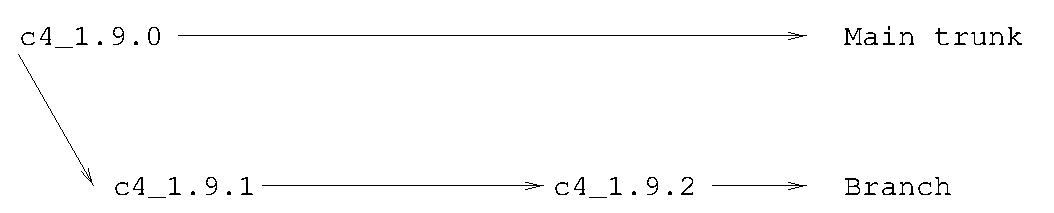
\includegraphics[width=4in]{branch.eps}}
  \caption{Schematic of a bug-fix branch in {\bf cvs}.}
  \label{fig:branch}
\end{figure}
following {\bf cvs} commands are used:
\begin{verbatim}
     cvs checkout -r draco-1_4_0 draco
     cd draco/src/c4
     cvs tag -b c4-1_9_1
\end{verbatim}
This creates a branch to \cfour\ release~1.4.  If the bug fix is
required in a \draco\ release, \draco\ should be re-released with the
appropriate branch number.  For example, to include
\texttt{c4-1\_9\_1} in a \draco\ release we tag \draco\ using:
\begin{verbatim}
     cvs checkout -r draco-1_4_0 draco
     cd draco/src
     cvs update -r c4-1_9_1 c4
     cd ..
     (run regression tests)
     cvs tag draco-1_4_1
\end{verbatim}
Thus, \draco\ itself is not put on a branch.  The branch number on
\draco\ versions indicates bug fixes in \draco\ packages.  %% Also note
%% that branches are, by definition, never in a \stable\ state.
Branches are used for bug fixes only.  %% Thus, a \stable\ release will
%% always be farther down the revision tree than a branch.

Additional fixes of bugs on package branches should be tagged using
\texttt{cvs tag c4-1\_9\_2}.  Thus, to make a tag to this \cfour\ 
version use the following commands:
\begin{verbatim}
     cvs checkout -r draco-1_4_1 draco
     cd draco/src
     cvs tag c4-1_9_2 c4
     cd ..
     (run regression tests)
     cvs tag draco-1_4_2
\end{verbatim}
We note that {\bf cvs} branches automatically release code to the end
of the branch.  Hence, \texttt{cvs checkout -r c4-1\_9\_1 c4} will
automatically give the sources at the end of the \cfour\ branch
connected to release~1.9.  We add tags to clarify the development and
bug tracking process in \draco\ even though they may not be strictly
necessary in all cases.  For more information on branches, see
Chapter~5 of the {\bf cvs} manual.

%%---------------------------------------------------------------------------%%

%% \section{Future Directions}
%% \label{sec:future}

%% \begin{itemize}
%% \item Move to git
%% \item Require bug tracking database
%% \item Description of code coverage and memory instrumentation
%%   requirements and tools.
%% \end{itemize}

%%---------------------------------------------------------------------------%%

\section{Summary}
\label{sec:summary}

The basic procedures explained in this document are robust.  However,
all procedures could benefit from future enhancements.  A list of
desired improvements to the \draco\ release procedures are:
\begin{itemize}
\item Release numbers in the \texttt{Release.cc} could be updated
  auto-magically through a script in the {\bf cvs} file
  \texttt{taginfo}.
\item {\bf cvs} major revision numbers could be updated auto-magically
  when the major release numbers on the tag are advanced.
\end{itemize}
These topics are noted for future consideration.

We have explained the release policies and procedures for
\draco\ projects in group CCS--2.  As with all \draco\ policies,
exceptions to the standard rules are acceptable pending review by
\draco\ team members.  These procedures have been reviewed and are
part of the \draco\ development process.

%%---------------------------------------------------------------------------%%

\bibliographystyle{rnote}
\bibliography{../../environment/bibfiles/draco}

\closing
\end{document}

%%---------------------------------------------------------------------------%%
%% end of draco-release.tex
%%---------------------------------------------------------------------------%%
